\subsection{Insertion frequency in fixed round windows}\label{app:pool-insertion-windows}

\Cref{fig:pool-insertion-windows} partitions the insertion history in
\cref{app:event-counters} into ten consecutive, nonoverlapping windows of
20 logged rounds. Every round contributes to exactly one window; the
first window starts at the committed admission history's first round.
The denominator is logged rounds, not candidate attempts or elapsed time.

\begin{figure}[tb]
  \centering
  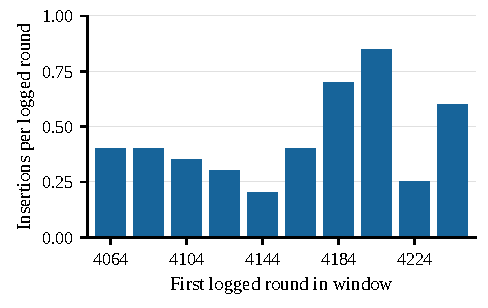
\includegraphics[width=\linewidth]{figures/fig_pool_insertion_windows.pdf}
  \caption{\textbf{Pool-insertion frequency varies across fixed round windows.}
  All ten nonoverlapping 20-round windows in rounds 4064--4263 of the
  committed history. Each bar is its exact insertion count divided by 20;
  the horizontal coordinate is the first round in that window. All 89
  insertions are retained. These engineering-event rates do not measure
  per-attempt success, wall-clock throughput or independent learning gain.
  Scope: \cref{sec:method-status}.}
  \label{fig:pool-insertion-windows}
\end{figure}
